\chapter{Introducción general}
\label{ch:introduccion}

Este capítulo presenta de forma breve el contexto del trabajo realizado.
Se explica la problemática solucionada y los conceptos necesarios para la lectura de la memoria.

\newcommand{\keyword}[1]{\textbf{#1}}
\newcommand{\tabhead}[1]{\textbf{#1}}
\newcommand{\code}[1]{\texttt{#1}}
\newcommand{\file}[1]{\texttt{\bfseries#1}}
\newcommand{\option}[1]{\texttt{\itshape#1}}
\newcommand{\grados}{$^{\circ}$}

\section{El espacio como recurso estratégico}
\label{sec:1space}

La explotación del espacio exterior permite mejorar la producción de bienes y servicios.
Además, provee datos de valor científico que incrementan la calidad de vida de las personas \citep{BOOK:spaceage}.
Finalmente, es una fuente de desafíos que impulsa el desarrollo tecnológico.

El marco jurídico que regula la explotación del recurso es el tratado sobre el espacio exterior de 1967.
Del cual, la República Argentina es miembro desde el 27 de enero de ese año.
Los países pueden reclamar cualquiera de las órbitas disponibles pero tienen la obligación de hacer uso dentro de un margen de tiempo determinado.
Luego, si el país no ocupó la órbita pierde el derecho a usarla \citep{BOOK:resurrect}.

El mercado de la explotación espacial está compuesto de estados y empresas.
Siendo las últimas quienes adquirieron el protagonismo en el siglo XXI \citep{ARTICLE:transition}.
El marco jurídico y la competencia en este rubro empujan a las compañías a innovar de forma permanente.
En particular, con nuevas técnicas y tecnologías que permitan abaratar el costo de las misiones.

El cliente de este trabajo es INVAP S.E. y es una empresa de la provincia de Río Negro.
La compañía es modelo en su tipo y realiza proyectos tecnológicos complejos en áreas como: reactores nucleares, satélites y radares.
En la figura \ref{fig:saocom} se puede observar un satélite realizado por la empresa.

\newpage

\begin{figure}[htbp]
	\centering
	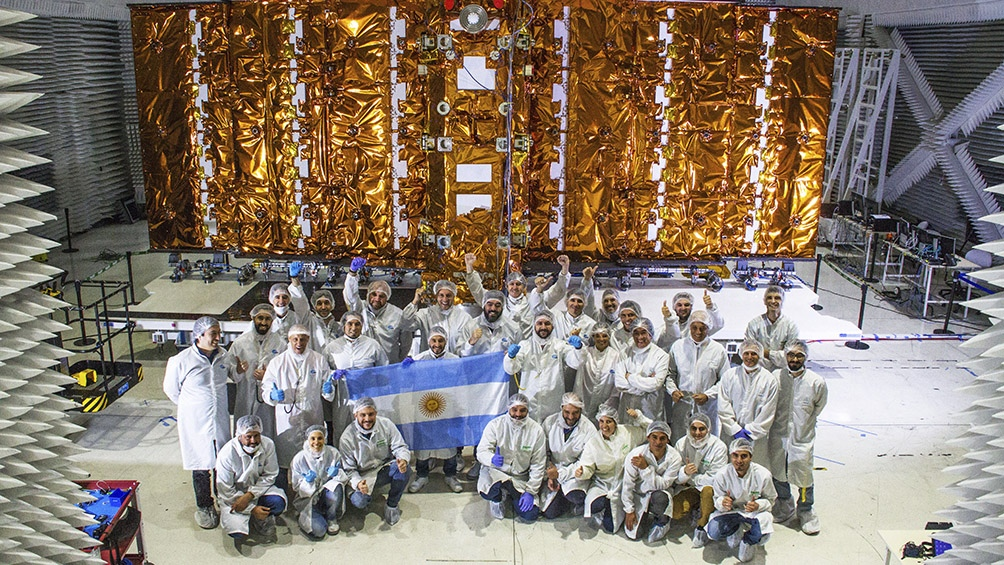
\includegraphics[width=\textwidth]{./Figures/invapsaocom.jpg}
	\caption{Satélite SAOCOM\protect\footnotemark.}
	\label{fig:saocom}
\end{figure}

\footnotetext{Imagen tomada de la página oficial de INVAP S.E. \citep{WEBSITE:invap}.}

\section{Radiación cósmica y sus efectos}
\label{sec:radiacion}

En el espacio hay tres fuentes de radiación ionizante de intensidad significativa:

\begin{itemize}
    \item Los electrones y protones que están atrapados en el campo magnético terrestre.
    \item Los protones e iones pesados que provienen del espacio interestelar.
    \item Los protones e iones pesados emitidos durante las fulguraciones solares.
\end{itemize}

La radiación es atenuada antes de llegar a la superficie del planeta gracias al campo magnético terrestre \citep{WEBSITE:structure_space_radiation}.
Como se puede ver en la figura \ref{fig:viento}, las partículas son desviadas y absorbidas por el campo.
Luego, este queda deformado y se genera una magnetosfera asimétrica.
En la tabla \ref{tab:capasmagneticas} se pueden observar las características de la asimetría.

\begin{table}[h]
	\centering
	\caption[Cinturón de Van Allen]{Cinturón de Van Allen \citep{WEBSITE:structure_space_radiation}.}
	\begin{tabular}{l c c}    
		\toprule
		\textbf{Cinturón} & \textbf{Frontera}           & \textbf{Partícula dominante}\\
		\midrule
		Interior          & 1,2 - 2,5 radios terrestres & Protones de alta energía\\		
		Exterior          & 2,8 - 12 radios terrestres  & Electrones de alta energía\\
		\bottomrule
		\hline
	\end{tabular}
	\label{tab:capasmagneticas}
\end{table}

La electrónica de los satélites se encuentra parcialmente blindada por las estructuras circundantes, sin embargo existe un alto grado de exposición a la radiación ionizante que se encuentra presente en su órbita.
Esto significa que la probabilidad de incidencia de una partícula cargada en el circuito es mayor.
La incidencia de una partícula genera una traza densa de pares electrón-hueco en los semiconductores \citep{ARTICLE:velazco}.
Además, es posible que esta ionización cause un pulso transitorio de corriente.

Los efectos de la radiación cósmica sobre el circuito pueden ser transitorios o permanentes.
Los permanentes se deben a la destrucción de una parte del circuito.
Esta destrucción es producto del disparo de componentes activos parásitos \citep{WEBSITE:effects_on_devices}.
Finalmente, en la tabla \ref{tab:radiacion} se puede ver un resumen de los tipos de errores generados por la radiación cósmica que de forma conjunta se denominan \emph{Single Event Effects (SEE)}.

Los cambios transitorios de estados internos de la electrónica dan lugar a lo que se denomina como \emph{soft-errors}, y son el objeto de estudio de este trabajo.
En la figura \ref{fig:bitflip} se puede ver el efecto transitorio de la radiación sobre los transistores de un integrado.
En particular, la inyección de un efecto denominado \emph{bit flip}.
Este se manifiesta como el cambio del valor de un bit en un registro o memoria.
La imagen muestra la colisión de una partícula cargada que excita e ioniza al semiconductor.
La línea punteada oblicua representa la traza de excitación que genera cambios en los campos eléctricos internos y altera los estados de conducción del dispositivo.
Luego, la activación de los transistores cambian los niveles de tensión en las señales de datos y control.
Finalmente, el circuito se normaliza pero con valores invertidos de tensión.

\begin{figure}[htbp]
	\centering
	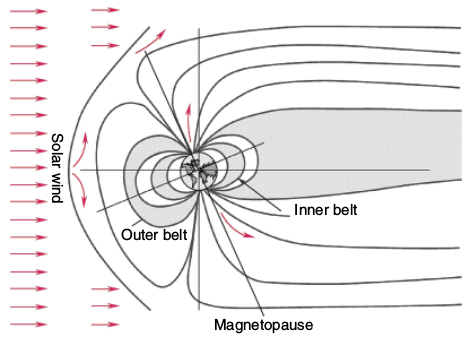
\includegraphics[width=0.8\textwidth]{./Figures/vientosolar.jpg}
    \caption{Capas magnéticas de la tierra y fulguración solar\protect\footnotemark.}
	\label{fig:viento}
\end{figure}

\footnotetext{Imagen tomada del artículo \emph{Structure of space radiation} \citep{WEBSITE:structure_space_radiation}.}

\begin{table}[h]
	\centering
	\caption[Efectos de la radiación cósmica]{Efectos producidos por la radiación cósmica \citep{WEBSITE:structure_space_radiation}.}
	\begin{tabular}{l c c}    
		\toprule
		\textbf{Evento}             & \textbf{Acrónimo} & \textbf{Efecto}\\
		\midrule
        \emph{Latch-up}             & SEL               & Pico de corriente destructivo\\		
        \emph{Upset}                & SEU               & Alteración de datos\\
        \emph{Funtional Interrupt}  & SEFI              & Cambios en la configuración\\
        \emph{Transient}            & SET               & Pico de tensión\\
		\bottomrule
		\hline
	\end{tabular}
	\label{tab:radiacion}
\end{table}

\newpage

\begin{figure}[htbp]
	\centering
	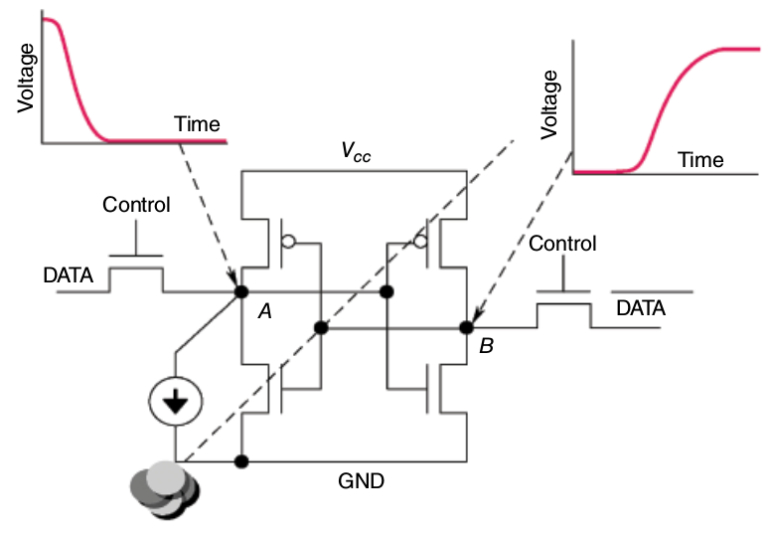
\includegraphics[width=0.8\textwidth]{./Figures/bitflip.jpg}
    \caption{Ejemplo simplificado de \emph{bit flip} en un bloque \emph{SDRAM}\protect\footnotemark.}
	\label{fig:bitflip}
\end{figure}

\footnotetext{Imagen tomada del artículo \emph{Effects of space radiation on electronic devices} \citep{WEBSITE:effects_on_devices}.}

\section{Calificación espacial e iniciativa \emph{New Space}}
\label{sec:newspace}

A los efectos vistos en la sección \ref{sec:radiacion} se suman: el estrés mecánico del lanzamiento y los cambios de temperatura en la órbita.
Este ambiente genera la necesidad de utilizar componentes con calificación espacial.
Para que un componente alcance la calificación espacial se debe someter a un largo y costoso proceso de acreditación.
Luego, estos componentes adolecen de un elevado precio y atraso tecnológico frente a los del mercado masivo \citep{ARTICLE:negocio}.

La irrupción del sector privado vista en la sección \ref{sec:1space}, trajo una nueva iniciativa comercial denominada \emph{New Space}.
Esta iniciativa busca bajar los costos al utilizar componentes no calificados para su uso espacial.
Además, existe la ventaja adicional de introducir tecnología de vanguardia.

El caso de Starlink es un ejemplo de \emph{New Space} particular.
Su volumen de satélites lanzados permite realizar conclusiones estadísticas significativas.
En particular, la presente dificultad para cumplir sus objetivos si se mantiene la actual tasa de mortalidad de sus satélites \citep{ARTICLE:cibils}.
En la figura \ref{fig:starlinkdeath} se puede observar que la constelación no lograría alcanzar la población deseada.
 
Al problema de población de Starlink se suma la gran cantidad de polución generada.
Los satélites fuera de servicio no pueden ser desorbitados y persisten en forma de \emph{debris}.
Como se puede ver en la tabla \ref{tab:starlinkdebris}, el volumen de basura generado es significativo.

\begin{table}[h]
	\centering
    \caption[Proyección de \emph{debris}]{Proyección de \emph{debris} de Starlink \citep{ARTICLE:cibils}.}
	\begin{tabular}{c c c c c}    
		\toprule
        \textbf{Lanzamientos} & \textbf{Satélites} & \textbf{Total lanzados} & \textbf{Población} & \textbf{\emph{Debris}}\\
		\midrule
        12                    & 60                 & 7200                    & 2704               & 4046\\		
        12                    & 180                & 21600                   & 8105               & 12146\\		
        12                    & 400                & 48000                   & 18007              & 26994\\		
        180                   & 60                 & 108000                  & 40000              & 61200\\		
        60                    & 180                & 108000                  & 40000              & 61200\\		
        27                    & 400                & 108000                  & 40000              & 61200\\		
		\bottomrule
		\hline
	\end{tabular}
	\label{tab:starlinkdebris}
\end{table}

\newpage

\begin{figure}[htbp]
	\centering
    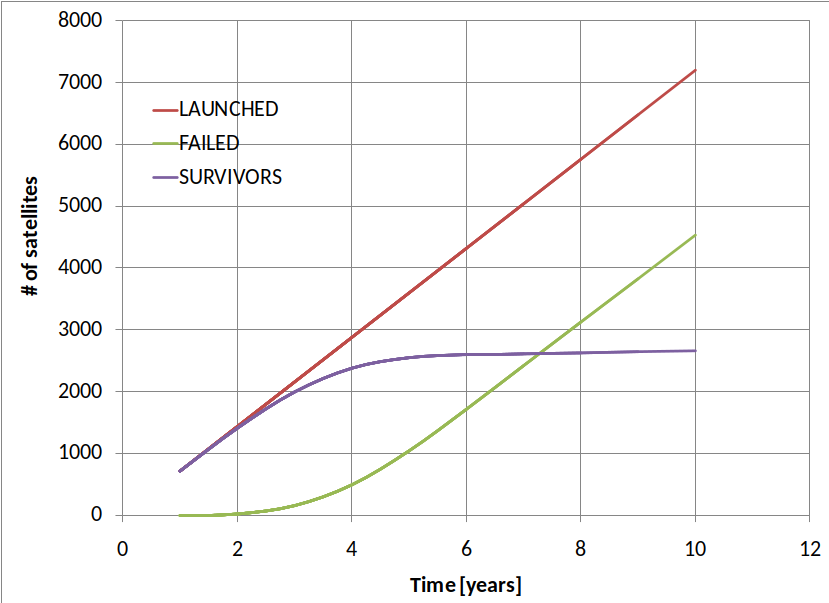
\includegraphics[width=\textwidth]{./Figures/starlinkpopulation.png}
    \caption{Proyección de la constelación Starlink\protect\footnotemark.}
    \label{fig:starlinkdeath}
\end{figure}
\footnotetext{Imagen tomada de la publicación de Roberto Cibils \citep{ARTICLE:cibils}.}

Las conclusiones del caso Starlink muestran la importancia de tener herramientas para simular el ambiente espacial.
En particular, los efectos de la radiación cósmica para poder probar las técnicas de mitigación de errores seleccionadas.
Finalmente, este trabajo agrega valor al cliente al incrementar la confiabilidad de los satélites y evitar los problemas de la competencia.

\section{Estado del arte}
\label{sec:arte}

La microelectrónica se encuentra en un proceso constante de cambio.
Se incrementa la densidad de integración, la velocidad de los dispositivos y se reducen los niveles de tensión eléctrica.
Este progreso hace que los circuitos sean más vulnerables a la radiación cósmica.

El uso de dispositivos sin calificación espacial hace que los riesgos frente a un error transitorio sean mayores.
Además, la aplicación final de vuelo no suele estar disponible durante la fase de desarrollo de los proyectos.
Esto dificulta aún más la mitigación de errores y aumenta la vulnerabilidad de los sistemas.

La manera tradicional de evaluar la tolerancia a los de errores de \emph{software} es realizar un ensayo por radiación.
En estos ensayos se utilizan instalaciones en tierra para pruebas de radiación.
Sin embargo, estas instalaciones son costosas y la preparación y ejecución de los ensayos consumen mucho tiempo.

Para lograr un ensayo por radiación, las instalaciones deben producir un haz de partículas cargadas.
Estas partículas se pueden obtener de:
\begin{itemize}
    \item Aceleradores de partículas: en esta categoría se incluyen ciclotrones y aceleradores lineales.
    \item Decaimiento por fisión: basados en el decaimiento por fisión espontánea de elementos como $Cf^{252}$.
\end{itemize}

En la figura \ref{fig:iones} se puede observar una cámara de iones pesados.
Durante el ensayo se ejecuta una metodología particular que define la actividad en el dispositivo bajo prueba.
Además, se necesita de un sistema que controle y observe el dispositivo bajo prueba durante su exposición a la radiación.
Finalmente, se requiere de personal calificado en el diseño, ejecución e interpretación de estos ensayos.

\begin{figure}[htbp]
	\centering
	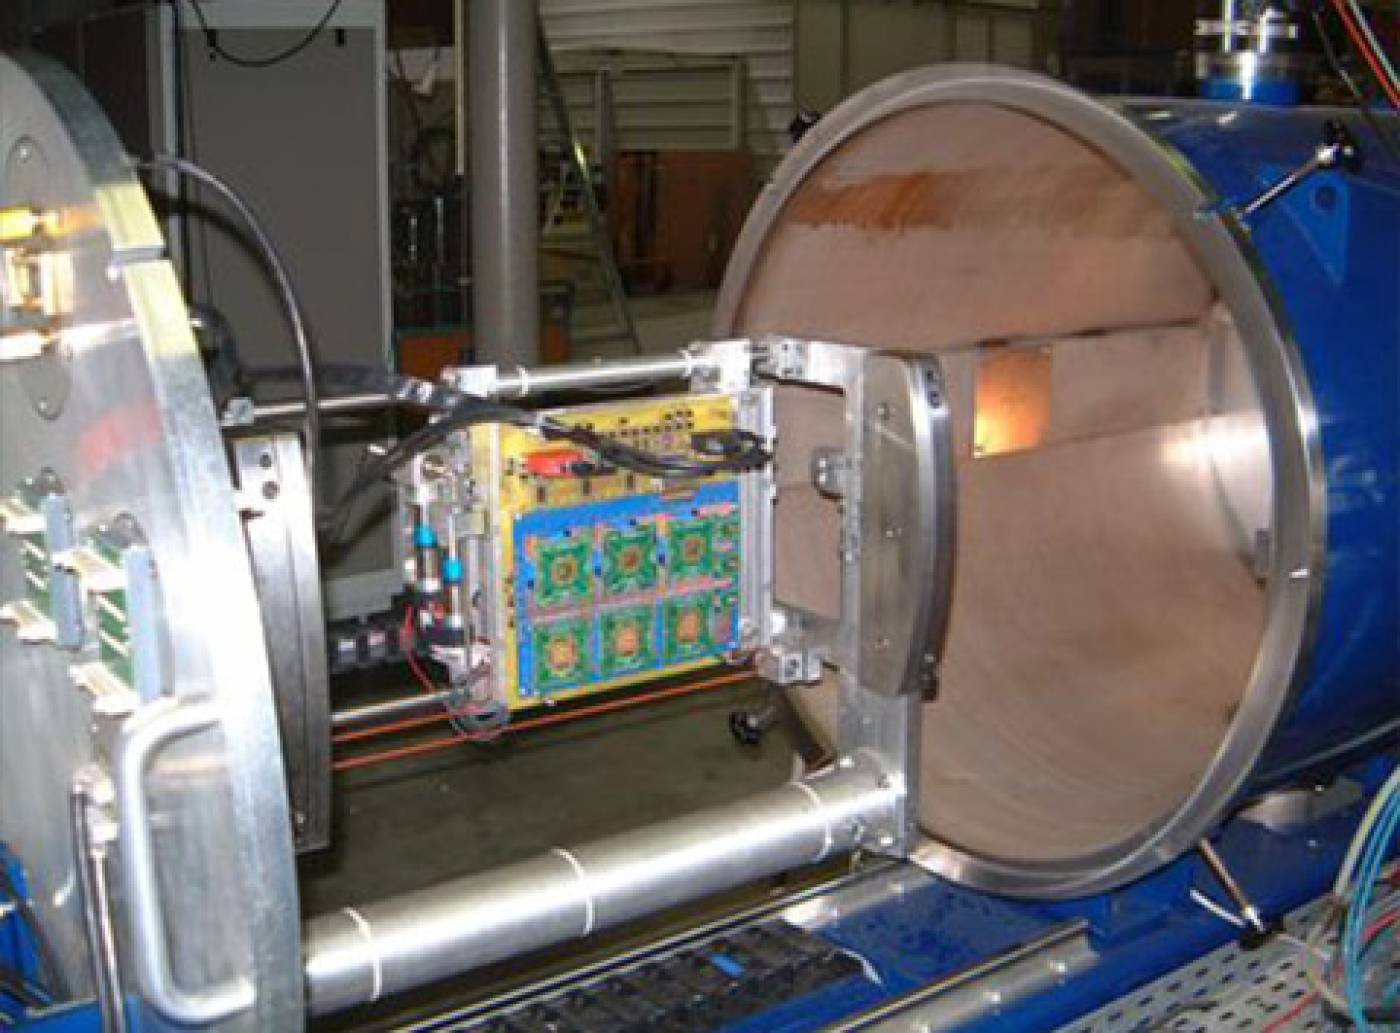
\includegraphics[width=\textwidth]{./Figures/heavy_ion_latchup_tests_in_louvain_la_neuve.jpg}
    \caption{Cámara de pruebas de iones pesados\protect\footnotemark.}
	\label{fig:iones}
\end{figure}

\footnotetext{Imagen tomada del sitio web ucl.ac.eu \citep{WEBSITE:heavy_ion}.}

Las estrategias para la inyección de errores pueden ser estáticas o dinámicas.
En las estáticas solo se observa si se producen cambios en valores determinados de memorias y registros.
Las pruebas dinámicas se realizan mientras se activan secuencias de lectura y escritura de memorias.
También incluyen la ejecución de programas para estimular el procesador.

El diseño de un ensayo dinámico necesita determinar la contribución de \emph{SEU} sobre una sección trasversal de memoria que está relacionada con su tiempo de lectura y escritura (ciclo de trabajo).
La sección trasversal de un programa se puede definir entonces como:

\begin{equation}
	\label{eq:crosssection}
    \sigma_{(SEU)} = \sum{d(R_i) \times \sigma_{R_i}}
\end{equation}

Donde:
\begin{itemize}
    \item $ d(R_i) $ es el ciclo de trabajo del elemento de memoria $ R $.
    \item $ \sigma_{R_i} $ es la sección transversal de memoria obtenida por la metodología estática \citep{ARTICLE:velazco}.
\end{itemize}

Diseñar un ensayo dinámico por radiación es un proceso largo y costoso, esto demanda que se distribuya la inversión de capital entre varias misiones.
Como consecuencia, el ensayo se realiza con un \emph{benchmark} que no representa realmente la aplicación de vuelo.
Finalmente, al ejecutar un ensayo genérico se obtiene un número mayor de \emph{soft-errors}.

Otra técnica disponible son los ensayos basados en \emph{software}, cuyo método se basa en emular la arquitectura a evaluar e introducir instrucciones que generen errores.
Esto genera un consumo de cómputo elevado y la problemática de estimar la tasa de error.
Con esta tasa se puede determinar en que momentos de la emulación corresponde introducir las instrucciones de error.
La tasa de error se estima como:

\begin{equation}
	\label{eq:errorrate}
    \tau_{SEU} = \sigma_{SEU} \times \tau_{inj}
\end{equation}

Donde $ \tau_{inj} $ es la tasa de incidencia de una partícula cargada.

Esta técnica demanda ciclos de la unidad de proceso y por lo tanto consume más tiempo de ejecución.
Además, cada vez que se altera el código fuente de la aplicación se necesita volver a diseñar una serie nueva de ensayos.

Existe una tercera técnica de ensayo de errores transitorios.
Esta técnica está basada en \emph{hardware}; y en el caso de los microprocesadores, se utiliza una sonda de depuración.
La principal ventaja de este método frente al basado en \emph{software} es que un mismo ensayo puede ser utilizado para múltiples iteraciones del código fuente.
Esto se debe a que la tasa de ocurrencia de los eventos nucleares sigue un proceso Poisson.
Si se observa el proceso como el tiempo que tarda en producirse cada impacto de una partícula cargada, entonces el proceso sigue una distribución exponencial.
Este razonamiento está sustentado en la siguiente ecuación:

\begin{equation}
	\label{eq:poisson}
    P(N_{SEU}(t + \Delta t) = N_{SEU}(t) ) = e^{-\sigma \times \phi \times \Delta t}
\end{equation}

El trabajo realizado es una solución del tipo ensayo por \emph{hardware}.
Además, se propuso superar el estado del arte de este método al crear una abstracción para el diseño de ensayos.
Los métodos mencionados presentan compromisos de ingeniería y están resumidos en la tabla \ref{tab:arte}.

\begin{table}[h]
	\centering
	\caption[Comparación de métodos de simulación]{Comparación de métodos de simulación \citep{ARTICLE:velazco}.}
	\begin{tabular}{l c c c}    
		\toprule
        \textbf{Método}        & \textbf{Eficiencia} & \textbf{Costo} & \textbf{Limitación}\\
		\midrule
        \emph{Software}        & Baja                & Bajo           & Ciclos de CPU\\		
        \emph{Hardware}        & Media               & Medio          & Acceso al integrado\\
        Radiación              & Alta                & Alto           & Control del ensayo\\
		\bottomrule
		\hline
	\end{tabular}
	\label{tab:arte}
\end{table}

\section{Alcance del trabajo}
\label{sec:alcance}

El trabajo realizado se divide en dos partes:
\begin{enumerate}
    \item \emph{Firmware} para el dispositivo bajo prueba.
    \item Inyector de \emph{soft-errors} por consola de comandos.
\end{enumerate}

El \emph{firmware} en el dispositivo bajo prueba tiene la misión de validar su funcionamiento.
Esto se logró al verificar cada periférico de interés dentro del integrado.
Luego, se generan reportes periódicos que se envían al inyector por consola de comandos.

En la figura \ref{fig:dutsimple} se puede observar un diagrama en bloques simplificado.

\begin{figure}[htbp]
	\centering
	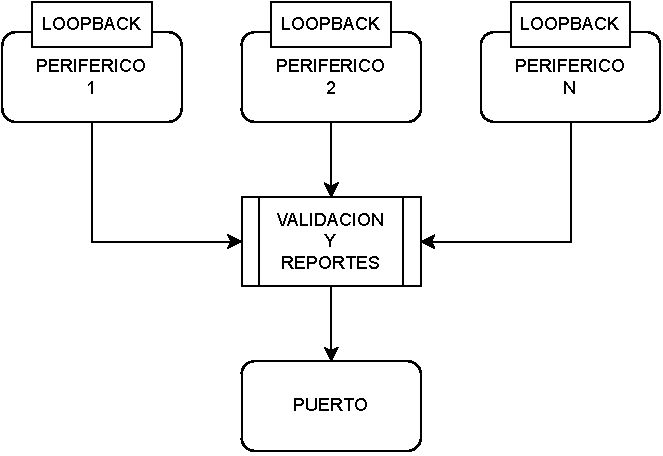
\includegraphics[width=\textwidth]{./Figures/dutsimple.pdf}
    \caption{Diagrama simplificado del dispositivo bajo prueba.}
	\label{fig:dutsimple}
\end{figure}

El inyector por consola de comandos tiene la función de planificar los ensayos y gestionar la introducción de errores.
En la figura \ref{fig:sisesimple} se puede ver como interactúan las partes del sistema.

\begin{figure}[h!]
	\centering
	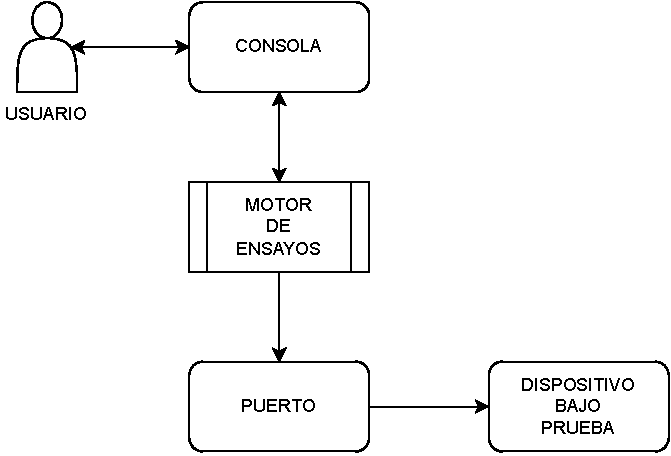
\includegraphics[width=\textwidth]{./Figures/sisesimple.pdf}
    \caption{Diagrama simplificado del sistema de inyección de errores.}
	\label{fig:sisesimple}
\end{figure}
\vspace*{3in}

